\chapter{Discussion}
Cellular life exists under conditions where the concentrations of nutrients, growth factors and oxygen are in constant flux. The dynamic instability of extracellular conditions requires that biological catalysts are highly efficient so that essential chemical compounds are generated at sufficient concentrations from the available extracellular nutrient pool. Moreover, the rate of chemical synthesis must be tightly controlled to maintain cellular homeostasis in response to signalling cues. Allostery is an important feature of enzyme regulation, which is potent and highly specific, and contributes towards maintaining organised flux through cellular pathways. Despite the ubiquity and demonstrated importance of allosteric regulation, an understanding of its mechanisms at the molecular level is limited, as is the curration of proteome-wide data on allosteric proteins.
%
%
\\\\
%
%
A detailed description of the regulatory mechanisms of PKM2 is relevant for understanding metabolic reprogramming in disease settings such as cancer, where it has been shown that inhibition of PKM2 activity can promote cancer cell growth by facilitating the provision of glucose-derived carbons for anabolic processes such as \textit{de novo} lipogenesis \cite{Anastasiou:2012aa}, serine biosynthesis \cite{Chaneton:2012aa}, nucleotide synthesis \cite{Kim:2015aa,Anastasiou:2012aa}, and the production of reducing equivalents such as glutathione \cite{Anastasiou:2011aa}. The discovery of a class of small molecules that activate PKM2 catalysis \cite{Walsh:2011aa,Boxer:2010aa,Jiang:2010aa}, and the finding that these small molecule activators alleviate the progression of xenograft breast tumours \cite{Anastasiou:2012aa}, support the hypothesis that exogenous regulation of PKM2 activity acts on a metabolic vulnerability of cancer cells \cite{Vander-Heiden:2011aa,Dayton:2016ab,Israelsen:2015aa,Vander-Heiden:2009aa}. Given the cancer-associated role of PKM2 regulation, knowledge of the molecular processes by which ligand binding incites changes to enzyme activity are of therapeutic interest. 
%
%
\\\\
%
%
In addition to feed-forward activation by fructose 1,6-bisphosphate (FBP), PKM2 is regulated by a number of other endogenous ligands, including the amino acids L-serine (Ser; an allosteric activator) \cite{Eigenbrodt:1983aa} and L-phenylalanine (Phe; an allosteric inhibitor) \cite{Feliu:1976aa}. Investigations into PKM2 regulation, thus far, have focused on the effects of individual ligands \textit{per se} on the structure \cite{Anastasiou:2012aa,Dombrauckas:2005aa,Yuan:2018aa,Gavriilidou:2018aa}, function \cite{Anastasiou:2012aa,Chaneton:2012aa,Christofk:2008aa} and dynamics \cite{Naithani:2015aa,Yan:2016aa,Zhong:2017aa} of PKM2. It is unclear whether ligands that concurrently bind to distinct allosteric pockets elicit in functionally independent effects, or whether the binding of multiple allosteric ligands with opposing functional signals produces a synergistic response.
%
%
\\\\
%
%
Here I offer evidence that PKM2 regulation constitutes a functional cross-talk between the effects of FBP and amino acids, which act in a combinatorial manner to modulate the allosteric transition of the tetrameric form of the protein between the inactive and active states. Using a novel method for predicting allosteric hub residues, \textit{AlloHubMat}, a network of protein residues is identified that couple FBP binding with enhanced substrate affinity. Moreover, two residues (A327 and C358) are identified that facilitate the cross-talk between FBP and Phe. 

\clearpage

\section{PKM2 is concurrently regulated by multiple allosteric ligands in a range of cellular conditions}
\label{discussion:cell_conditions}
An investigation into PKM2 regulation was initiated by determining the binding affinity of PKM2 to its endogenous regulators. An apparent dissociation constant in the nano-molar range [$K_{D}^{FBP}$ = (21.4 $\pm$ 9.0) nM] was estimated from measurements of FBP binding to PKM2 (Section \ref{subsec:fbp_binding_pkm2}). Tight binding between FBP and PKM2 resulted in purified recombinant PKM2 retaining substoichiometric amounts of \textit{E. coli}-derived FBP throughout the purification, despite extensive dialysis (Section \ref{subsec:fbp_binding_pkm2}). Amounts of co-purified FBP were quantified in all purifications of PKM2 and found that as much as 75 \% of the protein was pre-bound to the ligand (Section \ref{subsec:fbp_binding_pkm2}). Previous studies have reported co-purification of FBP with PKM2, suggesting a similarly high binding affinity as that reported here \cite{Christofk:2008aa,Morgan:2013aa,Gavriilidou:2018aa}. Our estimate of the binding affinity is in approximate agreement with that of Yan \textit{et al.} (2016) \cite{Yan:2016aa}: $K_{D}^{FBP}$ = 210 nM; and Gavriilidou \textit{et al.} (2018) \cite{Gavriilidou:2018aa}: $K_{D}^{FBP}$ = 910 nM. Neither publication, however, provide estimates of the amounts of FBP in the starting material of purified PKM2 and it is therefore unlikely that these studies account for the effect of ligand co-purification on the starting free protein concentration.
%
%
\\\\
%
%
The consequence of tight binding between FBP and PKM2 has been overlooked, thus far, as it raises questions regarding the biological role of FBP as an allosteric regulator of PKM2. To this end, intracellular concentrations of FBP were measured under fully-fed and glucose-deprived culture conditions in three human cancer cell lines (Section \ref{subsec:ic_concentrations}). Our findings revealed that intracellular FBP concentrations far exceeded the concentration of ligand required to achieve full saturation of PKM2. Consequently, under steady-state growth conditions, a significant fraction of PKM2 is predicted to be bound to FBP, even in the background of other regulatory stimuli such as post-translational-modifications, that influence FBP binding \cite{Christofk:2008aa,Hitosugi:2009aa} (Section \ref{subsec:pm2tide_kinetics}). 
%
%
\\\\
%
%
A protein concentration of 5 $\mu$M was used to measure the fluorescence spectrum of PKM2 and thereby monitor FBP binding (Section \ref{subsec:fbp_binding_pkm2}), which was approximately 240-fold greater than the calculated FBP binding affinity. Ideally, the concentrations of protein and ligand used for binding experiments should be in the same range as the measured $K_D$. Owing to the low quantum yield of tryptophan in intrinsic PKM2 fluorescence measurements, it was necessary to use PKM2 concentrations in the low $\mu$M range in order to obtain measurements with acceptable signal-to-noise ratios. Furthermore, PKM2 is a notoriously 'sticky' protein with a tendency to bind to the walls of the tube. While for many of the assays it was possible to avoid this (use of coated tubes, minimal sample mixing) diluting PKM2 to low concentrations for fluorescence measurements leads to significant loss of protein that makes such conditions unsuitable. 
%
%
\\\\
%
%
With these considerations in mind, the question is: can we derive meaningful $K_D$ values from our binding data? Simulations of ligand-receptor binding, and fitting of these data with the quadratic expression in Equ. \ref{equ:mass_action}, found that as the free protein concentration increases, the \% error in calculating the $K_D$ also increases and reaches 130 - 175 \% at protein concentrations 240-fold in excess of the binding affinity (similar to our experimental conditions in measuring FBP-PKM2 binding). This observation also reflects the large experiemental error reported for the $K_D$ of FBP for PKM2 (48 \%). Nevertheless, in spite of the large error associated with this measurement, due to the experimental limitations detailed above, we are still able to determine a range and an upper limit for the $K_D$ values we measure. The upper-limit of the FBP-PKM2 binding affinity, taking into account the theoretical percentage error, corresponds to 58 nM. Importantly, this upper limit is between 500- and 4000-fold lower that the measured intracellular concentration of FBP and therefore our assertion that PKM2 is saturated remains valid. This assertion is further supported by the persistence of FBP binding to purified PKM2 despite extensive dialysis during the process of purification. Furthermore, in addition to FBP binding to PKM2, we also determined the AC95, which indicates the concentration of FBP that results in 95 \% PKM2 activation, which we show is 529 nM i.e. 610-fold lower than the measured intracellular concentration (Section \ref{subsec:pkm2activity_subs_affinity}). 
%
%
\\\\
%
%
The notion that FBP is constitutively bound to PKM2 under a range of extracellular glucose conditions (0 mM - 11 mM) is supported by the finding that addition of exogenous FBP had little effect on PKM2 activity assayed in cell lysates, cultured both in fully-fed and glucose-starved conditions (Section \ref{subsec:cell_lysate_act_fbp}). Moreover, exogenous addition of phenylalanine to HCT116 cell lysates resulted in a dose-dependent decrease in the $k_{cat}$ (Section \ref{subsec:cell_lysate_act_fbp}), rather than an increase in the $K_{M}^{PEP}$ observed when purified recombinant PKM2 activity was assay upon addition of phenylalanine (Section \ref{subsec:phe_ser_fbp_activity}). While seemly contradictory, Phe inhibition of recombinant purified PKM2 in the presence of saturating concentrations of FBP was found also to reduce the $k_{cat}$, revealing an alternate mechanism of inhibition by Phe, and possibly other inhibitory amino acids, in the presence of constitutively bound FBP (Section \ref{subsec:phe_ser_fbp_activity}), further supporting the hypothesis that, under the presently tested cell culture conditions, PKM2 is constitutively bound to FBP. Additionally, our results show that competition between activating (Ser) and inhibiting (Phe) amino acids determines the rate of product turnover of PKM2, while constitutive FBP binding maintains the protein in a high-substrate affinity state (Section \ref{subsec:phe_ser_fbp_activity}). 
%
%
\\\\
%
%
Other amino acids L-alanine (Ala), L-tryptophan (Trp) and L-cysteine (Cys) have previous been shown to inhibit PKM2 activity \textit{per se} in the same way as Phe \cite{Yuan:2018aa}. Therefore, competition between activating and inhibitory amino acids may provide a potent mechanism of feed-forward activation and feed-back inhibition of FBP-bound PKM2 activity (\textbf{Fig. \ref{fig:pkm2_aa_model}}). Under conditions of high PKM2 activity, glucose-derived phosphoenolpyruvate is rapidly converted to pyruvate, expanding the intracellular pool size of pyruvate. Excess pyruvate can then be consumed by a number of reactions including reduction by lactate dehydrogenase to form lactate, or oxidation by pyruvate dehydrogenase to form acetyl-CoA. Alternatively pyruvate can be used as a substrate by one of the alanine aminotransferase enzymes. Alanine aminotransferase 1 (GPT)-catalysed transamination between pyruvate and glutamate forms $\alpha$-ketoglutarate and alanine (\textbf{Fig. \ref{fig:pkm2_aa_model}}). Accumulation of the alanine pool would feed-back inhibit FBP-bound PKM2 (PKM2$^{FBP}$), likely by the same hyperbolic-mixed mechanism observed for phenylalanine. Sustained allosteric inhibition of PKM2$^{FBP}$ would result in the accumulation of glycolytic intermediates, leading to utilisation of 3-phosphoglycerate for \textit{de novo} serine biosynthesis. Subsequent accumulation of serine would feed-forward activate PKM2  (\textbf{Fig. \ref{fig:pkm2_aa_model}}), as shown by Chaneton \textit{et al.} (2012) \cite{Chaneton:2012aa}. The findings presented herein, which support the idea that PKM2 is constitutively saturated with the activator FBP, suggest that serine-induced activation does not act to increase the substrate affinity of PKM2. Rather, high concentrations of serine, relative to the concentrations of alanine and other inhibitory amino acids, would act to out-compete the inhibitory amino acids from the amino acid binding pocket on PKM2, thereby alleviating the negative effect on the $k_{cat}$. Given that Phe, Ser, Ala, His and Trp bind to a common allosteric pocket \cite{Yuan:2018aa}, it is likely that their relative, rather than absolute, concentrations determine the activity of FBP-bound PKM2 (\textbf{Fig. \ref{fig:pkm2_aa_model}}). Whether intracellular flux through lower glycolysis is determined by the ratio between activating-to-inhibiting amino acid ligands is beyond the scope of this thesis, and warrants further investigation.
%
%
%%% FIGURE
%
\begin{figure}[!ht]
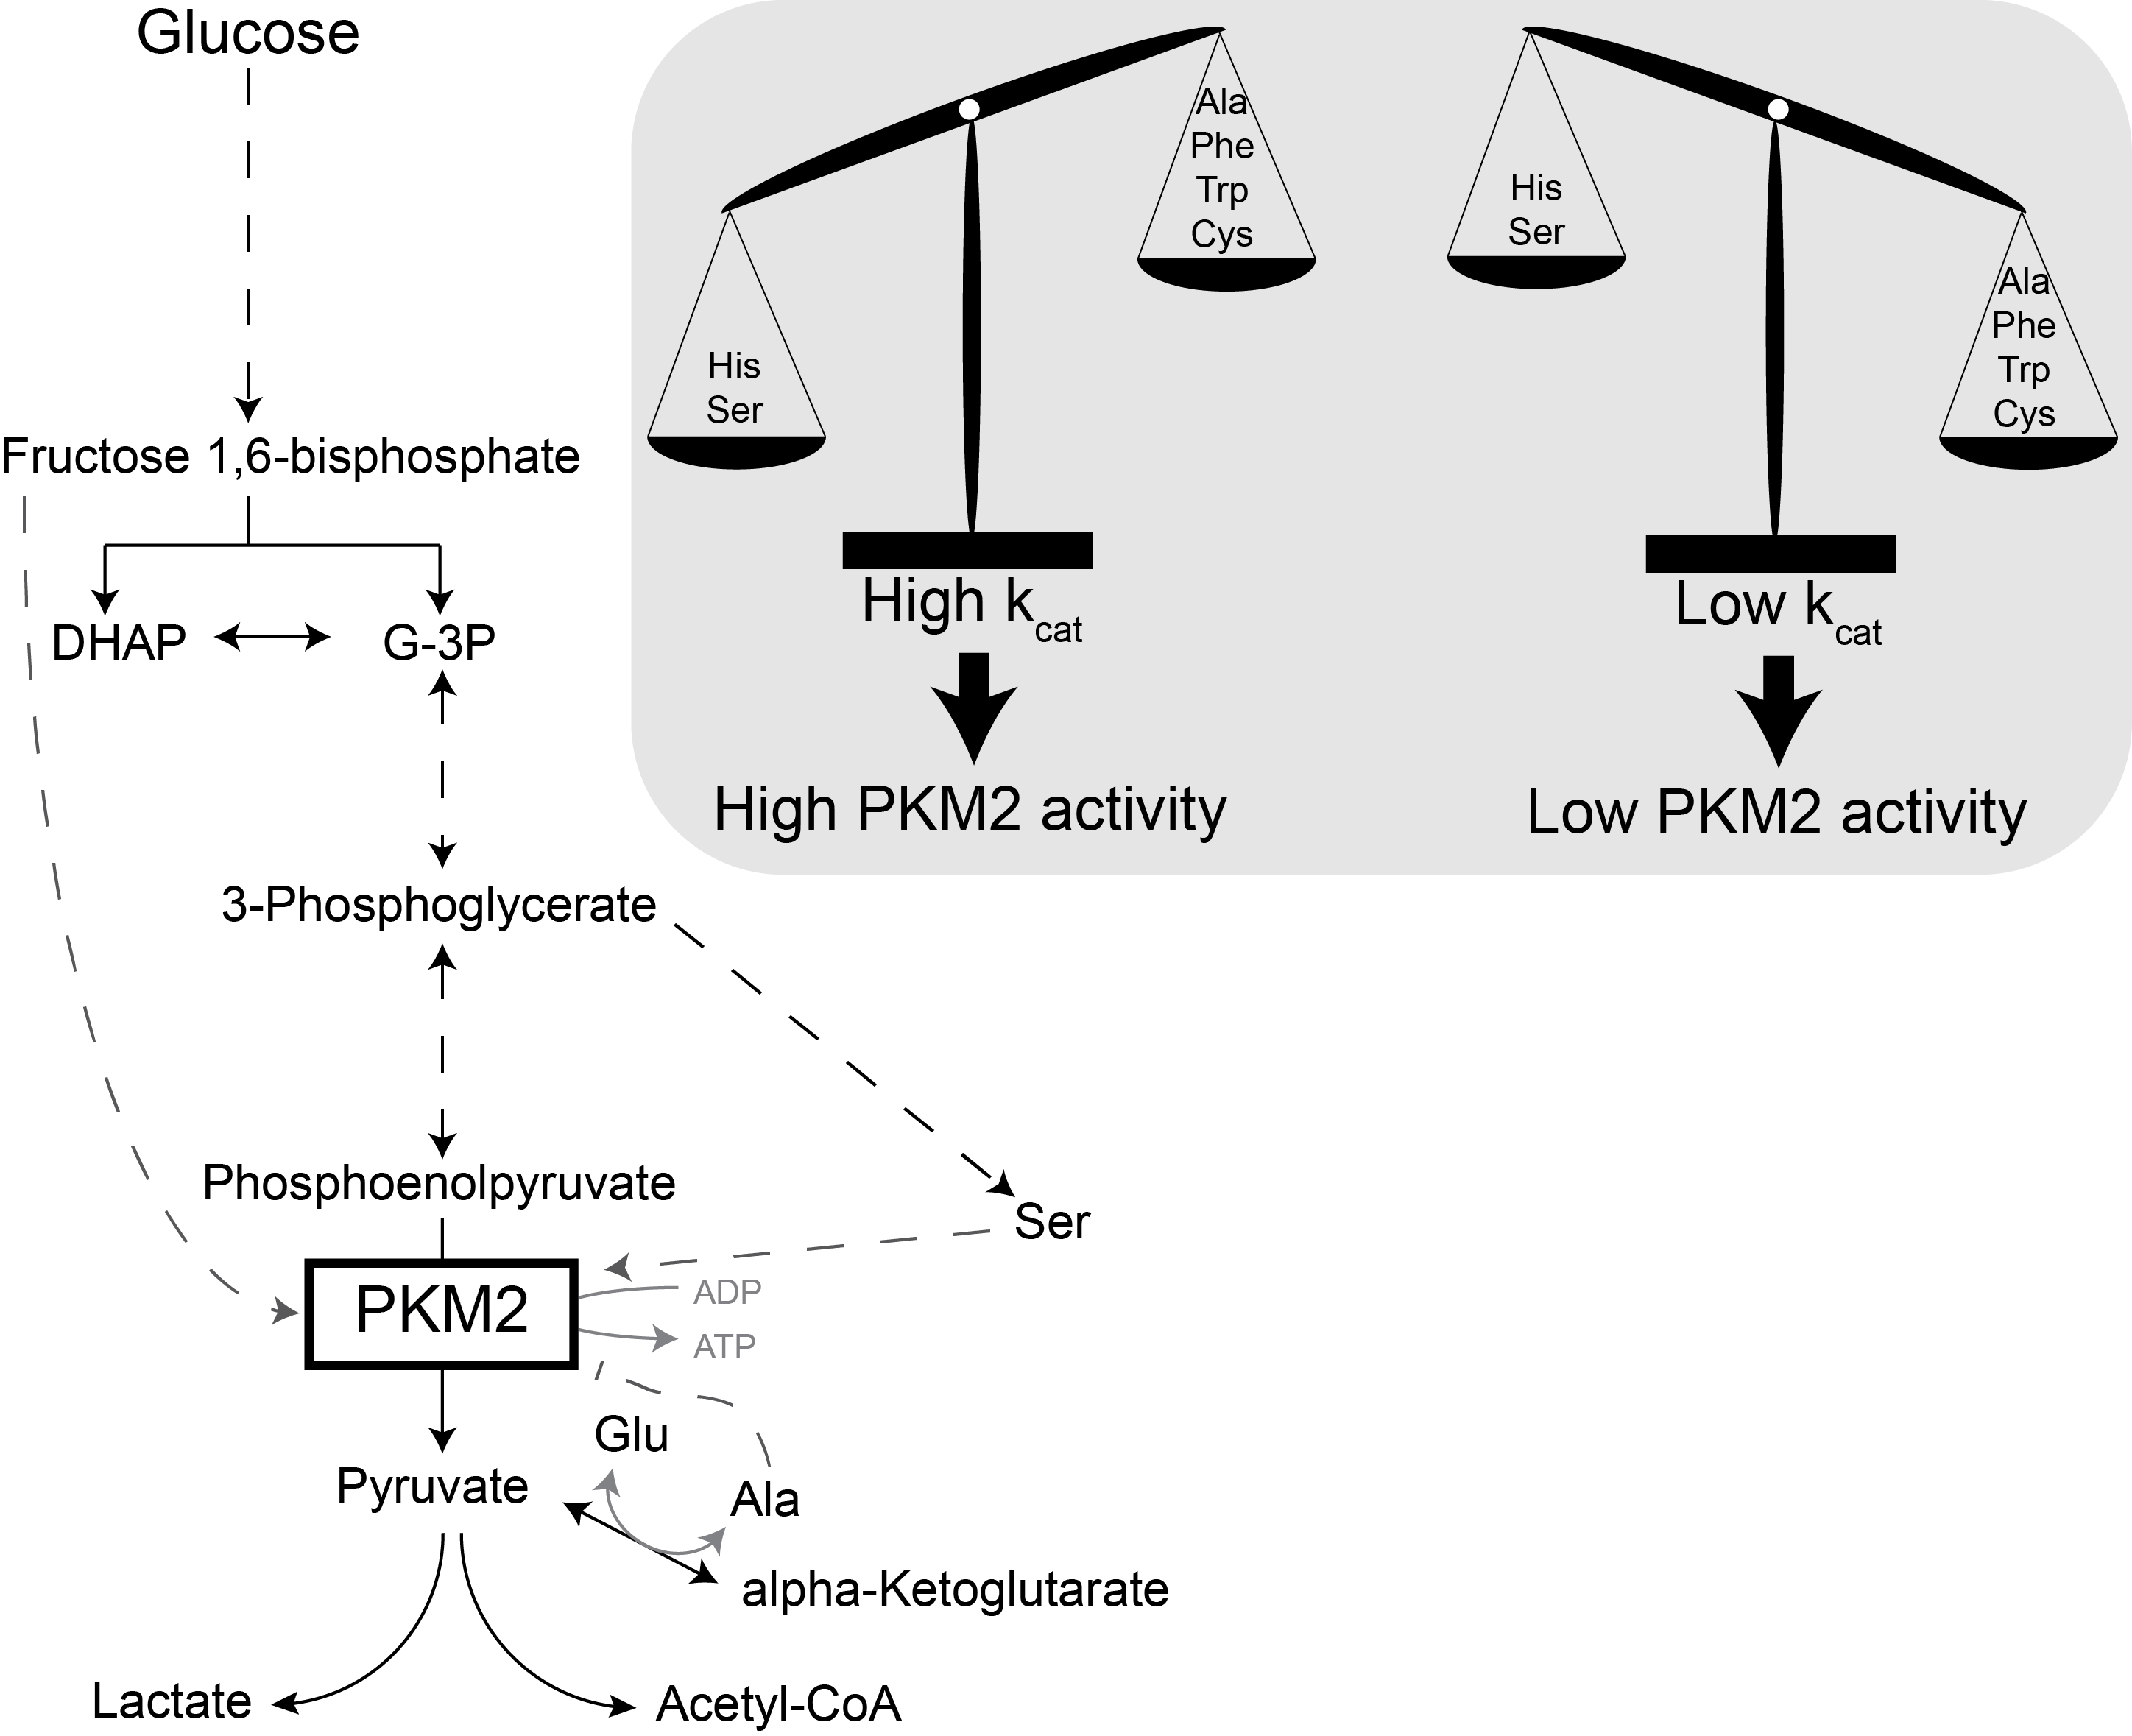
\includegraphics[scale=0.6]{pkm2_aa_scheme.png}
\caption[Proposed model of PKM2 regulation by amino acids.]{\textbf{Proposed model of PKM2 regulation by amino acids.} Work presented herein suggests that FBP is constitutively bound to PKM2, thereby locking the enzyme in a high-substrate affinity state. PKM2 enzyme activity can subsequently be regulated by activating and inhibitory amino acids which collectively compete for a single binding site. Therefore, high concentrations of inhibitory amino acids relative to activating amino acids, would act to reduce the rate of product turnover through a hyperbolic-mixed allosteric mechanism. Conversely, high concentrations of activating amino acids, relative to the pool size of inhibitory amino acids, would result in a high $k_{cat}$ by alleviating the effect of inhibitory amino acids.}
\label{fig:pkm2_aa_model}
\end{figure}
%
%
\clearpage

 
\section{FBP and Phe regulate PKM2 through a functional cross-talk}
The proposed model of PKM2 regulation outlined in Section \ref{discussion:cell_conditions} is supported by the finding that, while FBP and Phe bind to spatially distinct pockets on PKM2, both ligands influence the mode of action of the other without reciprocal effects on their binding affinities. The ability of Phe to perturb FBP-induced activation, suggests a functional cross-talk between the allosteric mechanisms of FBP and Phe. Previous studies have suggested that PKM2 enzyme activity is correlated with oligomerisation \cite{Hofmann:1975aa,Anastasiou:2012aa,Morgan:2013aa,Yuan:2018aa,Gavriilidou:2018aa,Feliu:1976aa,Eigenbrodt:1983aa,Ikeda:1998aa}. Therefore, to explore whether the combined effects of concurrent FBP and Phe regulation could be explained by changes to the oligomeric state of the protein, native mass spectrometry (MS) was used as a means to study the oligomeric structure and dynamics of PKM2 in the gas phase (Chapter \ref{chapter:mass_spec}).
%
%
\\\\
%
%
Native spectra of PKM2 revealed that the protein adopts a mixed population of monomers, dimers and tetramers (Section \ref{subsec:apo_pkm2_nms}). FBP addition was found to promote tetramerisation (Section \ref{subsec:fbp_tetramerisation}), in agreement with a recent native MS study \cite{Gavriilidou:2018aa}. An integrative approach using ion-mobility MS and \textit{in vacuo} MD simulations found that the dimers in the native spectra were formed stably about the A-A' interface (Section \ref{subsec:aa_dimer_imms}), which implies that FBP binding induces dimer-dimer association about the C-C' interface. This is supported by a previous study showing that a G415R mutation prevents tetramerisation about the C-C' interface and is thereby insensitive to FBP-induced activation \cite{Yan:2016aa}. In contrast, Phe addition had the effect of preferentially stabilising the dimeric species of PKM2 (Section \ref{subsec:fbp_phe_nativems}). Our results thus support the concept that FBP-induced activation stabilises the tetrameric species, while Phe-induced inhibition promotes dimeric PKM2.
%
%
\\\\
%
%
The finding herein that Phe binding \textit{per se} destabilises tetramers is in agreement with previous studies \cite{Hofmann:1975aa,Feliu:1976aa}, and contests the findings of two recent reports suggesting that Phe, and several other amino acids, promote the formation of an inactive tense \textit{T-state} tetramer \cite{Morgan:2013aa,Yuan:2018aa}. Critically, our observation that concurrent addition of Phe and FBP synergistically promotes the formation of tetramers (Section \ref{subsec:phe_fbp_synergistic_tet}) raises the possibility that Phe-induced stabilisation of the inactive tetramer reported by Morgan \textit{et al.} (2013) \cite{Morgan:2013aa} and Yuan \textit{et al.} (2018) \cite{Yuan:2018aa} is confounded by the presence of residually co-purified FBP. Indeed Morgan \textit{et al.} (2013) \cite{Morgan:2013aa} generated a mutant variant R489A in order to "[abolish] FBP binding and [prevent] contamination by FBP, which is commonly bound during purification of the protein from Escherichia coli culture." Nevertheless, it is unclear whether partial FBP occupancy is accounted for in these studies, as the amounts of co-purified FBP in preparations of recombinant purified PKM2 are not reported. It is notable, therefore, that Morgan \textit{et al.} (2013) \cite{Morgan:2013aa} chose to test oligomerisation upon Phe addition with PKM2(WT) (partially FBP-bound) rather than with PKM2(R489A) (fully apo). Based on the findings presented herein, one might speculate that the stabilisation of PKM2 tetramers by Phe observed by Morgan \textit{et al.} (2013) \cite{Morgan:2013aa} and Yuan \textit{et al.} (2018) \cite{Yuan:2018aa} could be attributed to significant amounts of residually co-purified FBP from \textit{E. coli}, which we found to be as high as 78 \% of the concentration of purified PKM2 (Section \ref{subsec:fbp_binding_pkm2}). 
%
%
\\\\
%
%
In addition to allosteric effects on PKM2 oligomerisation, several studies have invoked inter-domain structural changes consequent to ligand binding \cite{Dombrauckas:2005aa,Gehrig:2017aa,Morgan:2013aa,Yan:2016aa,Yuan:2018aa}. To this end, ion mobility coupled to native mass spectrometry (IM-MS) measurements were used to compute the rotationally-averaged collision cross section ($^{DT}CCS_{He}$) of PKM2 as a measure of the conformational heterogeneity of the protein. FBP binding resulted in a subtle shift in the $^{DT}CCS_{He}$ distribution, favouring a more extended form of the protein (Section \ref{subsec:fbp_ccsd}). This was partially reversed by the simultaneous addition of both FBP and Phe, favouring a more apo-like $^{DT}CCS_{He}$ distribution (Section \ref{subsec:ccsd_phe_fbp}). The apparent ligand-induced changes in PKM2 ion mobility may indicate a conformational shift between the T-state (tense) and the R-state (relaxed) tetramer, as described previously by Morgan \textit{et al.} (2013) \cite{Morgan:2013aa} and Yuan \textit{et al.} (2018) \cite{Yuan:2018aa}. Although informative, it is difficult to relate changes in ion mobility with specific structural events. Therefore, to study the process of ligand-induced structural rearrangement, we turned to an \textit{in silico} thermodynamic model of PKM2 (Chapter \ref{chapter:md}).
%
%
\\\\
%
%
MD simulations of tetrameric PKM2 found that allosteric activators FBP and Ser induced a closure of the B-domain cap over the active site pocket, whereas simulations of PKM2$^{FBP+Phe}$ and PKM2$^{Apo}$ tetramers revealed an opening of the B-domain cap (Section \ref{subsec:tet_bdomain_closure}). The concept of PKM2 ligand-dependent B-domain cap dynamics is supported by high B-factors calculated fro atoms in the B-domain of a crystal structure previously published by Dombrauckas \textit{et al.} (2005) \cite{Dombrauckas:2005aa}. This hypothesis is supported by molecular dynamics simulations published by Gehrig \textit{et al.} (2017) \cite{Gehrig:2017aa} and by Naithani \textit{et al.} (2015) \cite{Naithani:2015aa}, both describing an FBP-induced closure of the B-domain. Nevertheless, high-resolution evidence of the simulated phenomena remains elusive. Small-angle X-ray scattering measurements of PKM2 tetramers by Yan \textit{et al.} (2016) \cite{Yan:2016aa} observed a small decrease in the radius of gyration upon addition of FBP from 43 \AA to 41 \AA . The authors attributed no significance to the observed FBP-induced change, stating that "binding of FBP did not significantly alter the $R_{g}$ of PKM2(WT)" \cite{Yan:2016aa}. In retrospect, however, it is tempting to speculate that this small change in the $R_{g}$ may reflect the B-domain cap closure in the T- to R-state tetramer transition. This could be addressed experimentally using methyl-TROSY (transverse relaxation optimised spectroscopy) NMR spectroscopy, which enables the study of the conformational dynamics of large biomolecular systems \cite{Rosenzweig:2014aa}. 

\clearpage


\section{AlloHubMat reveals residues that mediate the cross-talk between FBP- and Phe-induced allosteric regulation}
To identify residues that mediate allosteric regulation of PKM2, the conformational dynamics of PKM2 tetramers upon FBP addition were analysed using molecular dynamics simulations of PKM2$^{apo}$ and PKM2$^{FBP}$ tetramers. Building on a previous approach by Pandini \textit{et al.} (2012) \cite{Pandini:2012aa}, the mutual information between sampled conformational states from MD trajectories encoded in a coarse-grained representation within the framework of the M32K25 structural alphabet \cite{Pandini:2010aa}. Proteins have been shown both experimentally \cite{Salvi:2016ab,Markwick:2009aa,Guerry:2013aa} and computationally \cite{Schmidt:2017aa,Daura:2001aa} to sample distinct conformational sub-states. This sampling of phase space is relevant for allosteric regulation of enzyme activity \cite{Sol:2009aa,Kern:2003aa,Eisenmesser:2005aa,Salvi:2016aa}, leading to the prevailing view that protein dynamics and allosteric regulation are ensemble phenomena \cite{Motlagh:2014aa}. Therefore, explicitly identifying allosteric signals that are representative of the ensemble of protein sub-states is critical. To this end, a novel computational framework, named AlloHubMat (\textbf{Allo}steric \textbf{Hub} prediction using \textbf{Mat}rices that capture allosteric coupling) was developed to predict allosteric hub fragments from the network of dynamic correlated motions, based on explicitly identified conformational sub-states from multiple MD trajectories and obtain an ensemble-averaged mutual information network (Section \ref{sec:allohubmat_dev}).
%
%
\\\\
%
%
At its core, AlloHubMat uses the M32K25 structural alphabet (SA) as a low-dimensional representation of the torsional space accessible to proteins \cite{Pandini:2010aa}. Each fragment in the alphabet contains two angles and a torsion angle, and is partitioned into 25 states forming a discrete-state model of protein structure. Previous SAs have used a similar fragment-based representation in the form of a set of Cartesian coordinates (MSM2000) \cite{Micheletti:2000aa}, or a vectorial description of consecutive C$\alpha$ atoms (CGT2004) \cite{Camproux:2004aa}. The M32K25 SA has the advantage, compared to other SAs, of being derived from a density-based approach \cite{ankerst1999optics}, so that the most dominant conformations are highly populated with multiple states \cite{Pandini:2010aa}. Therefore, even relatively subtle changes in the protein backbone are captured by changes between states within the M32K25 model. AlloHubMat overcomes limitations of previous approaches \cite{Pandini:2012aa,Lange:2006aa} that do not account for how distal correlated motions may change in direction and magnitude as the protein samples distinct sub-states over the course of an MD simulation, and predicts networks of allosteric residues from MD simulations using a consistent numerical framework to measure time-dependent correlated motions. The approach used by AlloHubMat facilitates the extraction of consensus allosteric networks from replicate MD simulations of a protein in a given liganded state, and the comparison of the consensus networks between simulations of different liganded states.
%
%
\\\\
%
%
Analysis of MD simulations of tetrameric PKM2 with AlloMatHub identified a number of candidate fragments as allosteric hub fragments (AlloHubFrags; Section \ref{subsec:allohubfrag_ident}). Starting from a selection of allosteric hub fragments (AlloHubFrags), single-point mutant variants (\textbf{Fig. \ref{fig:pkm2_structure_allohubmuts} A}) were designed and tested for their enzymatic response to FBP binding. Mutagenesis of several of the hubs (I124G, F244V, K305Q, F307P and R489L) disrupted FBP-induced activation (Section \ref{subsec:allohubmuts_fbp}), demonstrating the utility of AlloHubMat for identifying \textit{bona fide} mediators of allostery. Of the five mutants that abrogated allosteric activation of PKM2, three mutants (F244V, F307P and R489L) disrupted the process of oligomerisation (Section \ref{subsec:allohubmut_ms}), suggesting that these AlloHubs mediate the FBP-induced monomer/dimer to tetramer transition (\textbf{Fig. \ref{fig:pkm2_structure_allohubmuts} B}). Conversely, AlloHubMuts I124G and K305Q maintained the ability to tetramerise upon FBP addition (Section \ref{subsec:allohubmut_ms}), though their allosteric activation was perturbed (Section \ref{subsec:allohubmuts_fbp}). Additional mutants of residues A327 and C358 preserved the allosteric coupling between FBP binding and enzyme activation, though prevented the inhibitory effect of Phe on PKM2$^{FBP}$ activity (\textbf{Fig. \ref{fig:pkm2_structure_allohubmuts} B}; Section \ref{subsec:allohubmuts_fbp}). The finding that A327S and C358A maintained wild type-like FBP activation but perturbed Phe inhibition indicated a role for these two residues in mediating a cross-talk between the allosteric mechanisms of Phe and FBP, which enables the inhibitory amino acid to inhibit the effect of FBP. C358 has been previously identified as an oxidation substrate of reactive oxygen species, whereby PKM2 can be post-translationally modified resulting in enzyme inhibition \cite{Anastasiou:2011aa}. None of the AlloHubMuts fell within residues 389-429 that differ between PKM2 (allosterically regulated) and the constitutively active splice-isoform (PKM1), suggesting that residues that confer differences in the allosteric properties of the two isoforms are dispersed throughout the protein structure. Zhong \textit{et al.} (2017) \cite{Zhong:2017aa} recently reported a synergistic mechanism whereby adenosine monophosphate (AMP) and glucose-6-phosphate (G6P) activate \textit{M. tuberculosis} pyruvate kinase. AMP binds to the equivalent of the FBP binding pocket, whereas G6P binds to a different pocket that is also distinct from the equivalent of the amino acid binding pocket on human PKM2. The synergistic mechanism between G6P and AMP is somewhat similar to the one described between FBP and Phe, here. Therefore, it is tempting to speculate that allosteric synergism upon concurrent binding of different ligands is a common mechanism of enzyme regulation.   
%
%
%%% FIGURE
%
\begin{figure}[!ht]
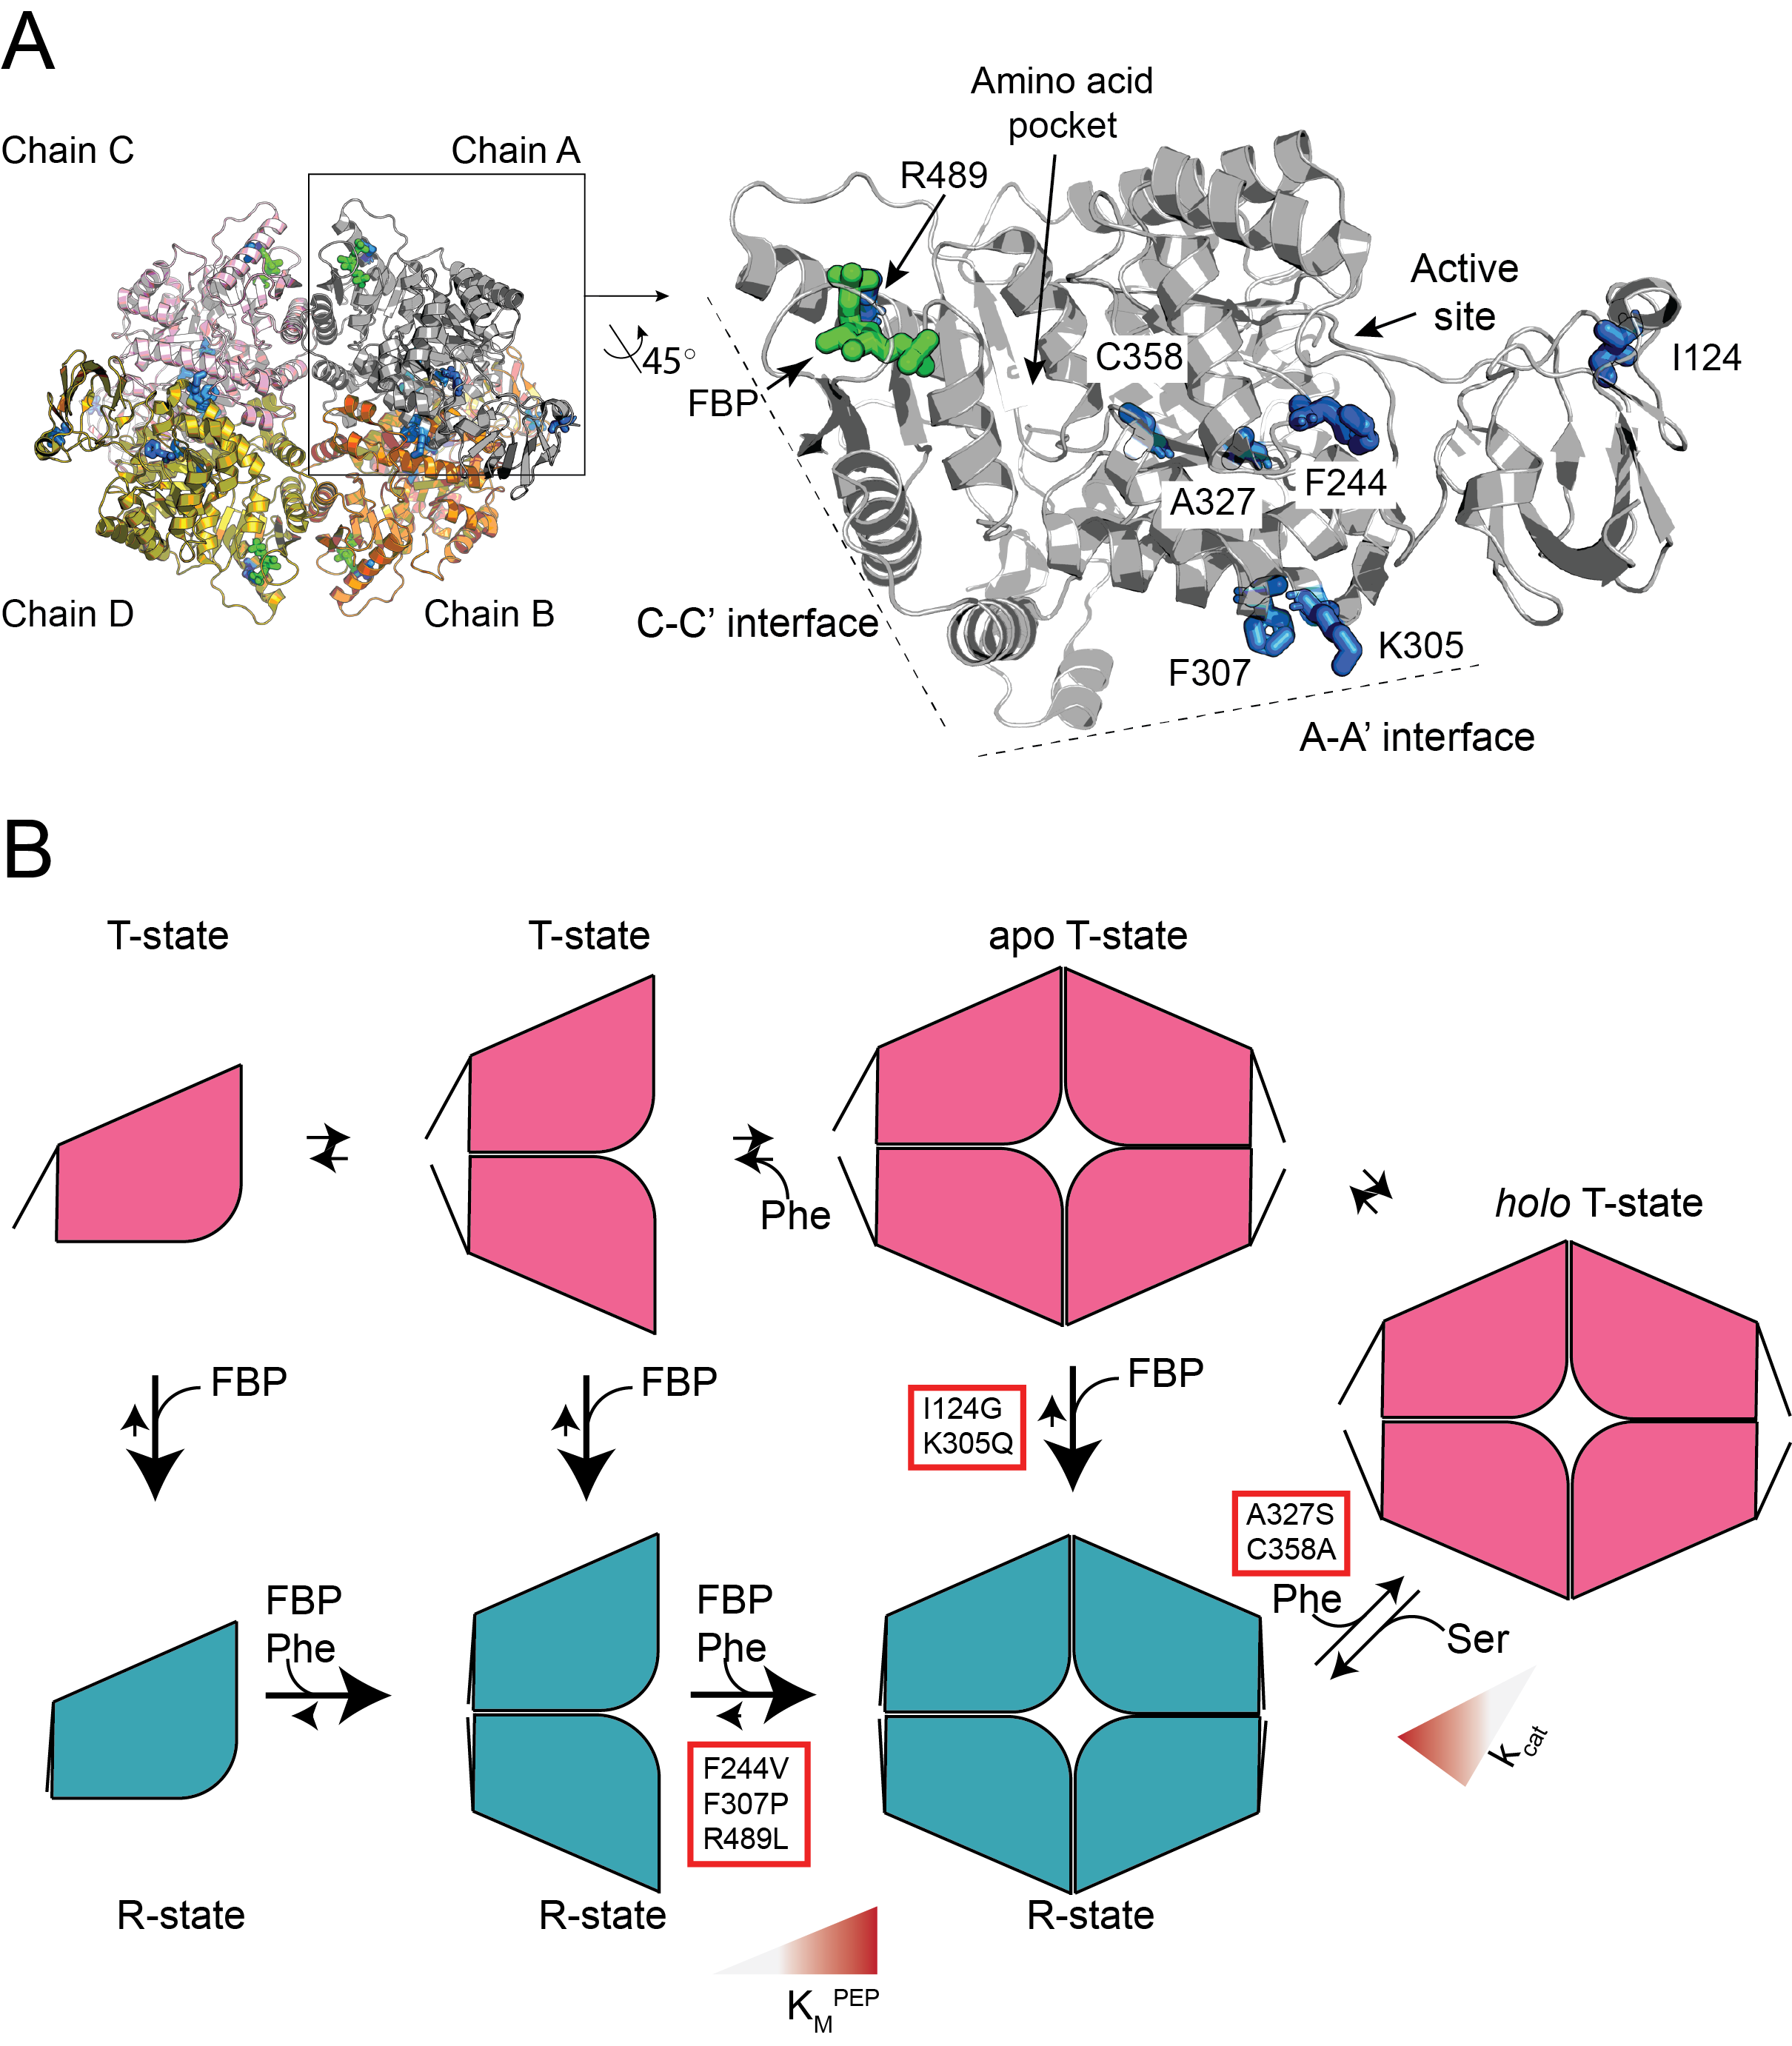
\includegraphics[scale=0.7]{allohubfrag_location.png}
\caption[The location and function of the AlloHubMuts.]{\textbf{The location and function of the AlloHubMuts.} \textbf{(A)} A structural schematic of PKM2 showing the location the seven AlloHub mutations (AlloHubMuts) on the protomer. The FBP molecule is shown in green and the locations of the amino acid binding pocket and the active site are annotated. \textbf{(B)} FBP-induced tetramerisation is propagated by a network of residues involving F244, F307 and R489. An apo T-state tetramer is populated in the ensemble of available states, to which FBP can bind, inducing a transition to the R-state tetramer. This T-state to R-state transition is accompanied by subtle conformational changes, likely involving the closure of the B-domain cap over the active-site pocket, which is correlated with an increased substrate binding affinity. The R- to T-state transition is mediated by I124 and K305, and mutations at these positions perturb the formation of a high substrate-affinity R-state tetramer.}
\label{fig:pkm2_structure_allohubmuts}
\end{figure}
%
%
\\\\
%
%
Evidence presented in Chaters \ref{chapter:md} and \ref{chapter:allohubmut} suggests that AlloHubMat is able to identify residues involved in the allosteric mechanism of an enzyme. Nevertheless, a recent large-scale alanine scanning mutagenesis study of liver pyruvate kinase (PKL) approximated that more than 30 \% of the protein residues are involved in its allosteric regulation \cite{Tang:2017aa}. Consequently, it can be argued that a statistical validation of AlloHubMat should focus on measuring the effect of mutating non-hub residues as negative controls for assessing the precision of the method. A comprehensive validation of the method was beyond the scope of this Thesis. Moreover, the mechanism enzyme regulation is likely case-dependent; for some proteins configurational entropy is the main driver of allostery \cite{Capdevila:2017aa,Cooper:1984aa,Popovych:2006aa,Saavedra:2018aa,Tzeng:2012aa}, and for others enthapic motions dominate the allosteric transition \cite{Freiburger:2014aa,Hewitt:2016aa,Pacholarz:2017aa,Rosenzweig:2014aa,Volkman:2001aa,Webb:2015aa}. This reasoning would conclude that a case-by-case validation of methods to predict allosteric regulation is required, which largely defeats the purpose of a predictive computational method. Moreover, high-throughput analyses of protein allostery using site-directed mutagenesis is compounded by the challenging task of purifying a very large number of mutant variants and investigating whether the introduced chemical perturbations abrogate coupling between distal sites, oligomerisation, or both. To this end, proteome-wide curation of data resulting from the experimental characterisation of enzyme mutants would address the outstanding challenge of benchmarking AlloHubMut and other computational methods for predicting allosteric hubs. 
%
%
\\\\
%
%
The spatial resolution of AlloHubMat is currently limited to fragments of four successive C$\alpha$ atoms. In Chapter \ref{chapter:md}, single-point mutants were designed from four-residue candidate hubs, based on an empirical analysis of the per-residue conservation within the identified hubs. In addition to identifying hub fragments, it would be desirable to explicitly identify the residue(s) within a hub fragment that contribute most to ochestrating the allosteric mechanism. Given that neighbouring fragments were found to be correlated, it was not possible to derive the per-residue mutual information using the chain rule for mutual information (Section \ref{subsec:allohubfrag_ident}). Future developments could improve the resolution of AlloHubMat by incorporating other sequence-based \cite{Lockless:1999aa,Tesileanu:2015aa} and statistical mechanical \cite{Guarnera:2016aa,Guarnera:2017aa,Tee:2018aa} methods, to build a combined predictive score. Sequence-based methods to measure residue co-evolution of distal residues \cite{Juan:2013aa} have been highly successful in predicting allosteric pathways in a number of cases \cite{McLaughlin:2012aa,Reynolds:2011aa}, and would add chemical and evolutionary information that is lost in our coarse-grained approximation of protein dynamics.

\clearpage

\section{Conclusion}
Allosteric regulation of PKM2 by FBP has long been viewed as a prototypical example of feed-forward regulation in biology, though the molecular mechanism of FBP activation remained largely elusive. PKM2 is additionally regulated by a plethora of endogenous ligands including several amino acids. It has been unclear, thus far, how PKM2 integrates the signals elicited by concurrently bound ligands, and the functional consequences of multi-ligand binding. To this end, the allosteric mechanism of PKM2 was investigated using an integrative computational and experimental approach. 
%
%
\\\\
%
%
Estimations of the fraction of intracellular PKM2 bound to its ligands found that that FBP concentrations far exceed that, which is required for full saturation of PKM2. Under steady-state growth conditions, a significant fraction of PKM2 is already bound to the activator FBP, even in the context of other regulatory cues, such as PTMs, that may influence ligand binding. Constitutive PKM2-FBP binding implicated FBP as an 'allosteric co-factor', rather than a reversible activator of PKM2 catalysis, raising questions regarding how PKM2 activity is regulated in the context of saturating FBP. Subsequent to FBP binding, amino acids Phe and Ser were found to reversibly modulate the maximal velocity of FBP-bound PKM2, suggesting an important role of amino acid regulation in lower glycolysis.
%
%
\\\\
%
%
Simultaneous Phe and FBP binding was found to synergistically promote PKM2 tetramerisation, despite the two ligands revealing opposing effects on oligomerisation \textit{per se}, revealing a functional cross-talk. To unravel the atomic basis by which allosteric coupling between distal sites is propagated within a protein, a novel computational method \textit{AlloHubMat} was developed. Analysis of molecular dynamics simulations using AlloHubMat, and extensive experimental characterisation of candidate mutant variants, found that the process of FBP-induced activation is propagated by a network of residues involving I124, F244, K305, F307 and R489. Moreover, mutations of A327 and C358 were found to perturb the effect of Phe on FBP-induced activation, thus revealing molecular details of the FBP-Phe cross-talk.
%
%
\\\\
%
%
In summary, results herein reveal that PKM2 integrates multiple allosteric inputs to regulate enzyme activity. This phenomenon is analogous to multiple-input-single-output (MISO) controllers in control system engineering, which integrate multiple transmission signals (allosteric ligands) and relay a single signal to a receiver (enzyme activity). Beyond PKM2, it is likely that many more proteins in the cell possess the ability to bind to multiple regulatory ligands. Though whether a systems-control mechanism of integrating the inputs from multiple ligands is a general property of such proteins is unknown. Identifying allosteric hubs using AlloHubMat to design mutants that perturb the allosteric response of proteins to individual, or multiple, ligands presents a powerful toolbox for the study of both the mechanistic basis of allosteric signal integration as well as the functional consequences of combinatorial allosteric inputs on enzyme regulation. 


\clearpage

























